\documentclass[a4paper,12pt]{article}
\usepackage[T1]{fontenc}
\usepackage[utf8]{inputenc}
\usepackage{geometry}
\geometry{a4paper, margin=1in}
\usepackage{lmodern}
\usepackage{listings}
\usepackage{xcolor}
\usepackage{hyperref}
\usepackage{setspace}
\usepackage{graphicx}
\usepackage{enumitem}

\setlist{itemsep=0pt}
\setlength{\parindent}{0pt}
\lstset{
    backgroundcolor=\color{gray!10},
    basicstyle=\ttfamily,
    numbers=left,
    numberstyle=\tiny,
    frame=single,
    breaklines=true,
    showstringspaces=false
}

\begin{document}

\begin{titlepage}
    \centering
    \vspace*{2cm}
    
    {\Huge \textbf{CYLite Compiler Project} \par}
    \vspace{0.5cm}
    {\Large \textbf{Language Specification and Grammar Modifications Report} \par}
    
    \vspace{3cm}
    
    {\Large \textbf{Authors:} \par}
    \vspace{0.3cm}
    {\Large Tejas Lohia \par} % You can edit your name or add your partner's name here
    {\Large [Shardul Junagade / 23110297] \par} 
    {\Large [Swayam Borate / 23110066] \par} 
    
    \vspace{2cm}
    {\large \textbf{CS327 Compilers - Lab Assignment} \par}
    
    \vfill
    
    {\large \today \par}
\end{titlepage}

\tableofcontents
\newpage

\setstretch{1.4}
\section{Introduction}

The landscape of programming languages has long been divided between highly performant, statically typed systems languages like C, and highly expressive, dynamically typed scripting languages like Python. C provides unparalleled control over hardware and memory layout, executing with optimal efficiency. However, its syntax can be unforgiving; error handling relies heavily on cumbersome return codes, control flow can become deeply nested and difficult to read, and iterative constructs often lead to off-by-one errors. Conversely, Python offers ergonomic syntax, explicit error handling blocks, and intuitive looping mechanisms, but at the cost of execution speed and strict compile-time type safety. 

CYLite represents a modern hybridization of these two paradigms. It is designed as an extension of the YAPL (Yet Another Programming Language) baseline compiler, effectively injecting Python-inspired syntactic sugar and control flow structures into a C-style language grammar. The fundamental motivation behind CYLite is to provide developers with the readability and expressiveness of modern high-level languages without sacrificing the structural rigor of a statically compiled environment. 

Developing a formal grammar for CYLite requires adapting these high-level programming concepts into a strictly unambiguous LALR(1) framework compatible with compiler generation tools like GNU Bison. By integrating these features directly at the lexical and grammatical level—rather than relying on standard library macros or external subroutines—the compiler pipeline can elevate them to first-class citizens in the language. This allows the compiler front-end to perform rigorous syntax checking, generate more optimized Abstract Syntax Trees (ASTs), and produce clearer compile-time error messages tailored to the programmer's explicit intent. 

This project focused heavily on redefining the parser rules (\texttt{yapl.y}) to accommodate these new grammatical structures. By modifying the base YAPL grammar, we introduced several new nonterminal rules and shifted existing expressions to handle newly introduced keywords. Specifically, the grammar now natively understands chained conditional blocks (via \texttt{elif}), explicit null operations (via \texttt{pass}), native I/O primitives (\texttt{print}), ergonomic loop iterators (\texttt{foreach} and \texttt{in range}), and block-scoped error encapsulation (\texttt{try-except}). 

This structural evolution ensures that CYLite can parse declarative flow states seamlessly while resolving dangling-else ambiguities and iteration pitfalls inherent to older grammars. This report breaks down the philosophy behind each addition and details the exact grammatical transformations applied to achieve the CYLite language specification.

\singlespacing

\section{Grammar Modifications}

To implement the CYLite language extensions, the lexical analyzer (generated via Flex) was first updated to recognize new keywords and allocate corresponding tokens. The parser (\texttt{yapl.y}) was subsequently heavily modified to integrate these new tokens into valid syntax trees.

\subsection{Lexical Additions (Tokens)}
We introduced the following terminal tokens into the parser to represent the core vocabulary of the new language features:
\begin{itemize}
    \item \texttt{ELIF}, \texttt{PASS}, \texttt{TRY}, \texttt{EXCEPT}, \texttt{PRINT}, \texttt{RANGE}, \texttt{IN}, \texttt{FOREACH}
\end{itemize}

\begin{figure}[h!]
    \centering
    % Replace the placeholder below with your actual image filename
    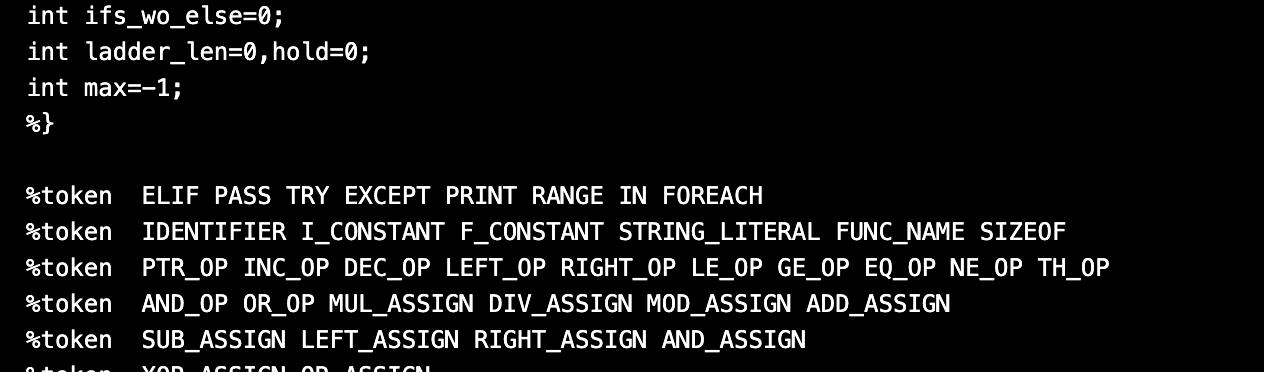
\includegraphics[width=0.8\textwidth]{./Images/imgh1.jpeg}
    \caption{Implementation of the new CYLite tokens in the lexical analyzer.}
    \label{fig:lexical_tokens}
\end{figure}


\subsection{The \texttt{elif} Conditional Construct}
In standard C, chaining conditionals often leads to deeply nested else-then-if forms, while the \texttt{else if} pattern is still treated as an \texttt{else} branch containing another \texttt{if} statement. In complex logical branching, this can disrupt readability and complicate AST generation due to classic dangling-else ambiguities. Python’s \texttt{elif} provides a unified, first-class construct for multi-way branching without artificial nesting.


\textbf{Grammar Change:} We defined a new nonterminal \texttt{elif\_list} to explicitly handle zero or more \texttt{elif} branches recursively. We then expanded \texttt{selection\_statement} to support an \texttt{if} block followed optionally by an \texttt{elif\_list} and a final optional \texttt{else}.

\begin{lstlisting}
elif_list
    : ELIF '(' expression ')' statement
    | elif_list ELIF '(' expression ')' statement
    ;

selection_statement
    : IF '(' expression ')' statement ELSE statement
    | IF '(' expression ')' statement
    | IF '(' expression ')' statement elif_list ELSE statement
    | IF '(' expression ')' statement elif_list
    ...
\end{lstlisting}

\subsection{Native Error Handling: \texttt{try-except}}
Error handling in C typically falls back to checking integer return codes after every function call, or using precarious \texttt{setjmp/longjmp} chains for global exits. Modern languages isolate fragile code within explicit boundaries, redirecting failures to localized catch blocks. By implementing \texttt{try-except} directly in the CYLite grammar, we establish dedicated scope blocks for execution and recovery, allowing the backend to map these to structured, object-level exception-handling routines.

\textbf{Grammar Change:} We introduced a \texttt{try\_except\_statement} combining the \texttt{TRY} keyword, a localized block (\texttt{compound\_statement}), the \texttt{EXCEPT} keyword, and its associative block. This nonterminal was then injected into the overarching \texttt{statement} rule.

\begin{lstlisting}
try_except_statement
    : TRY compound_statement EXCEPT compound_statement
    ;

statement
    ...
    | try_except_statement
\end{lstlisting}

\subsection{Ergonomic Iteration: \texttt{foreach} and \texttt{in range}}

Classic C \texttt{for} loops require boilerplate initialization, condition checking, and manual incrementation (e.g., \texttt{for(int i=0; i<10; i++)}). This pattern is verbose and inherently prone to off-by-one errors. CYLite adopts \texttt{foreach id in enumerable} and \texttt{for(id in range(a, b))} to abstract the iteration boilerplate. This makes the programmer's intent purely declarative rather than imperative, preventing out-of-bounds complications.

\textbf{Grammar Change:} The \texttt{iteration\_statement} nonterminal was expanded to natively parse these specialized loops, tying identifiers directly to iterable sequences and mathematical ranges.

\begin{lstlisting}
iteration_statement
    ...
    | FOR '(' IDENTIFIER IN RANGE '(' expression ',' expression ')' ')' statement
    | FOREACH '(' IDENTIFIER IN expression ')' compound_statement
\end{lstlisting}

\subsection{The explicit \texttt{pass} Operation}

In standard C, an intentionally empty block or stubbed function is often written as a pair of empty braces or a lone semicolon \texttt{;}. This is visually ambiguous, and compilers or semantic linters may flag it as a probable mistake. Promoting the explicit \texttt{pass} keyword provides an unambiguous syntactic placeholder, asserting that the empty block is intentional.

\textbf{Grammar Change:} \texttt{PASS ';'} was added directly as a terminal production alternative within the \texttt{statement} rule.

\begin{lstlisting}
statement
    ...
    | PASS ';'
\end{lstlisting}

\subsection{First-Class \texttt{print} Built-in}

Rather than relying exclusively on importing \texttt{stdio.h} to use the variadic \texttt{printf} function—which requires cumbersome format strings and type awareness—CYLite promotes basic output to a native built-in language feature. By integrating it into the grammar, \texttt{print} can be more strictly type-checked or implicitly optimized for polymorphic output at compile-time by the parser's AST builder without requiring external linkage headers.

\textbf{Grammar Change:} The \texttt{print} construct was appended defensively to \texttt{postfix\_expression}, supporting both empty calls and list arguments.

\begin{lstlisting}
postfix_expression
    ...
    | PRINT '(' ')'
    | PRINT '(' argument_expression_list ')'
\end{lstlisting}

\subsection{Results}
The integration of these advanced features required careful consideration of LALR(1) parsing constraints to avoid shift/reduce and reduce/reduce conflicts within the Bison generator framework. By directly extending the \texttt{yapl.y} grammar definitions, CYLite successfully bridges the architectural gap between systems programming and scripting conveniences. Developers can now write highly readable, python-inspired code while leaning on the reliable, rigorous syntax-checking rules inherent to a C-like toolchain.

\newpage
\section{Automaton Generation and Initial Analysis}

To construct the LALR(1) item sets and build the parser automaton (fulfilling Part 1 of the assignment requirements), we processed the modified \texttt{yapl.y} grammar file using GNU Bison.

\subsection{Bison Invocation and Outputs}
The parser generator was invoked using the following command:
\begin{lstlisting}
$ bison -v -d yapl.y
\end{lstlisting}

This command utilizes two critical flags:
\begin{itemize}
    \item \textbf{\texttt{-d}:} Generates the \texttt{yapl.tab.h} header file, which exposes the newly defined CYLite terminal tokens (e.g., \texttt{ELIF}, \texttt{FOREACH}, \texttt{TRY}) to the Flex lexical analyzer.
    \item \textbf{\texttt{-v} (Verbose):} Instructs Bison to generate a detailed \texttt{yapl.output} file. This file is crucial as it contains the human-readable representation of every LALR(1) item set and the complete state transition graph for the automaton.
\end{itemize}

\subsection{Initial LALR(1) Automaton Analysis}
The generation process successfully constructed the LALR(1) automaton required to parse the CYLite language specification. An initial analysis of the generated \texttt{yapl.output} report reveals the following structural metrics regarding the grammar's complexity:
\begin{itemize}
    \item \textbf{Grammar Rules:} The parser implements over 130 distinct production rules to encapsulate both the core C-style expressions and the advanced CYLite extensions.
    \item \textbf{Item Sets (States):} The resulting LALR(1) automaton consists of 522 distinct states (item sets). This large state space is a direct result of the complex expression precedence and the newly introduced deeply nested control structures (such as \texttt{try-except} and \texttt{elif} ladders).
\end{itemize}

While the item sets and state machine were successfully compiled, the integration of optional branching (specifically the \texttt{elif} and \texttt{else} derivations) and ambiguous operator precedence introduced non-determinism into the parsing table. The initial Bison compilation reported exactly \textbf{6 shift/reduce conflicts} and \textbf{1 reduce/reduce conflict}. The identification, isolation, and resolution of these conflicts are documented in the following section.


\subsection{Conflict Identification and Resolution}

As noted in the initial automaton analysis, the introduction of CYLite's advanced control structures—specifically the \texttt{elif} ladders and optional \texttt{else} blocks—introduced non-determinism into the LALR(1) parsing table. When processed by GNU Bison, the grammar generated exactly 6 shift/reduce conflicts and 1 reduce/reduce conflict. 


\begin{figure}[h!]
    \centering
    % Replace the placeholder below with your actual image filename
    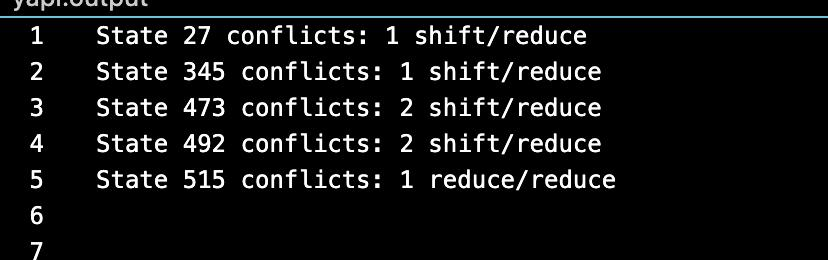
\includegraphics[width=0.8\textwidth]{./Images/image2.jpeg}
    \caption{Identification of the conflicting states in the LALR(1) automaton.}
    \label{fig:conflicting_states}
\end{figure}


To satisfy the structural rigor required by the compiler front-end, we must isolate the specific item sets where the automaton encounters multiple valid transition paths, identify the conflicting productions, and apply deterministic precedence rules to resolve them.

\subsection{Shift/Reduce Conflict: The \texttt{ATOMIC} Keyword Ambiguity}

One of the identified conflicts occurs in \textbf{State 27} and involves the \texttt{ATOMIC} keyword. This is a \textbf{Shift/Reduce conflict}.

\vspace{0.7cm}

\textbf{Exact Productions Involved:}

\begin{figure}[h!]
    \centering
    % Replace the placeholder below with your actual image filename
    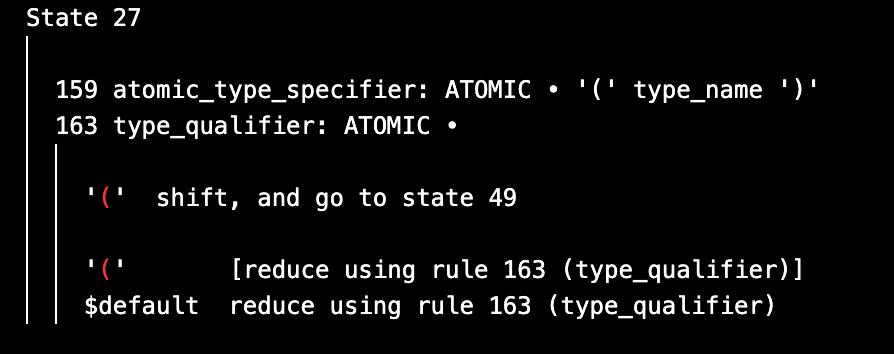
\includegraphics[width=0.8\textwidth]{./Images/image3.jpeg}
    \caption{Example of a shift/reduce conflict involving the \texttt{ATOMIC} keyword.}
    \label{fig:ifelse_dangling}
\end{figure}

\textbf{Conflict Analysis:}
In this state, the parser has just consumed the \texttt{ATOMIC} token and is looking ahead at the next token, which is an opening parenthesis \texttt{`('}. The automaton faces a structural ambiguity:
\begin{itemize}
    \item \textbf{Shift Action:} It can shift the \texttt{`('} token onto the stack, anticipating an \texttt{atomic\_type\_specifier} construct (e.g., \texttt{\textunderscore Atomic(int)}).
    \item \textbf{Reduce Action:} It can immediately reduce the \texttt{ATOMIC} token into a \texttt{type\_qualifier} (acting similarly to \texttt{const} or \texttt{volatile}), assuming the parenthesis belongs to a subsequent cast or expression.
\end{itemize}
Bison's default behavior resolves this by favoring the shift operation, but the conflict indicates a deeper grammatical overlap between qualifiers and type specifiers.

\subsection{Shift/Reduce Conflict: Abstract vs. Concrete Pointer Declarators}

Another significant conflict surfaces in \textbf{State 345}, representing a \textbf{Shift/Reduce conflict} driven by the overlap between named declarators and abstract type definitions, complicated by embedded semantic actions.

\begin{figure}[h!]
    \centering
    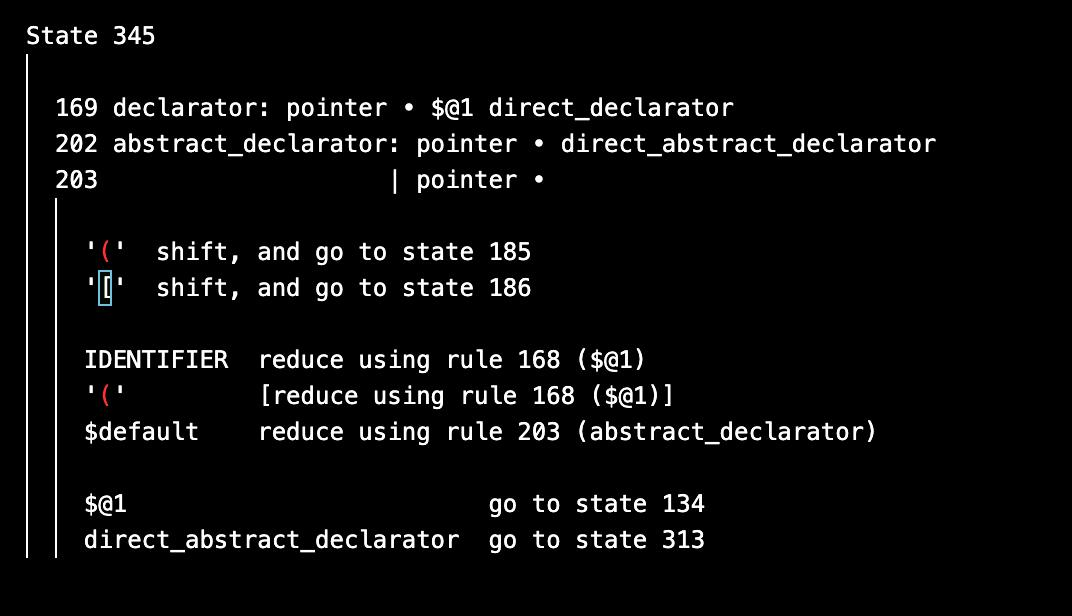
\includegraphics[width=0.8\textwidth]{./Images/image4.jpeg}
    \caption{Shift/Reduce conflict involving abstract and concrete pointer declarators in State 345.}
    \label{fig:pointer_conflict}
\end{figure}

\textbf{Conflict Analysis:}
In this state, the parser has processed a pointer token (e.g., \texttt{*}) and is looking ahead at an opening parenthesis \texttt{`('}. The ambiguity arises because the parser cannot immediately determine if it is parsing an \texttt{abstract\_declarator} (such as a typecast \texttt{(int *())}) or a concrete \texttt{declarator} (such as a variable declaration \texttt{int *(p)}). 

Crucially, the concrete \texttt{declarator} rule contains an embedded mid-rule semantic action (Rule 168 / \texttt{\$@1}), which increments the \texttt{pointer\_decls} counter. The automaton faces two conflicting choices:
\begin{itemize}
    \item \textbf{Shift Action:} Directly shift the \texttt{`('} onto the stack to begin constructing a \texttt{direct\_abstract\_declarator} (which lacks the mid-rule action).
    \item \textbf{Reduce Action:} Immediately reduce the empty mid-rule action \texttt{\$@1} (executing the counter increment) before shifting the \texttt{`('} to build a standard \texttt{direct\_declarator}.
\end{itemize}
Bison defaults to shifting, which means pointer declarations wrapped in parentheses might temporarily bypass the embedded semantic counter until the conflict is explicitly resolved.

\newpage




\subsection{Shift/Reduce Conflicts: The Dangling-Else and \texttt{elif} Ambiguity}

The most prominent structural ambiguities introduced by the CYLite extensions occur within the conditional branching logic, explicitly captured in \textbf{State 473}. This represents a classic \textbf{Shift/Reduce conflict} compounded by the new \texttt{elif} construct.

\textbf{Exact Productions Involved:}
\begin{figure}[h!]
    \centering
    % Replace the placeholder below with your actual image filename
    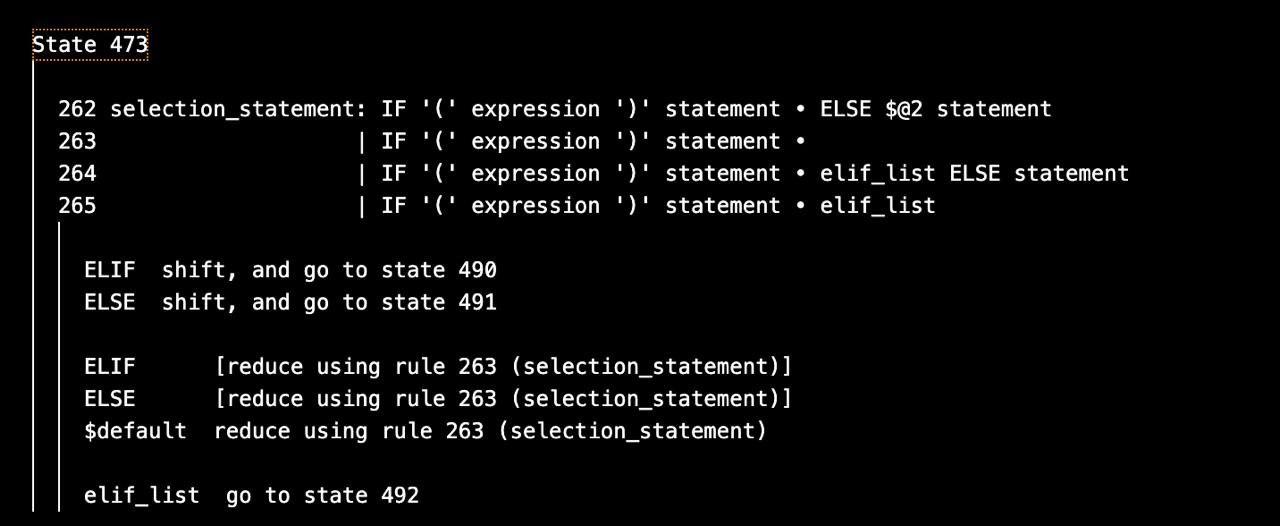
\includegraphics[width=0.8\textwidth]{./Images/image5.jpeg}
    \caption{Shift/Reduce conflict involving the Dangling-Else and \texttt{elif} ambiguity in State 473.}
    \label{fig:dangling_else_conflict}
\end{figure}


\textbf{Conflict Analysis:}
In State 473, the parser has successfully matched an entire \texttt{IF} statement up to its closing block (indicated by the dot \texttt{.} after \texttt{statement}). It is now looking ahead at the next token, which is either an \texttt{ELIF} or an \texttt{ELSE}. The automaton is trapped in a non-deterministic state due to the possibility of nested conditionals (e.g., \texttt{if (A) if (B) pass; else pass;}):
\begin{itemize}
    \item \textbf{Shift Action:} The parser can shift the \texttt{ELIF} or \texttt{ELSE} token onto the stack, aggressively binding it to the most recently opened (innermost) \texttt{IF} statement.
    \item \textbf{Reduce Action:} The parser can immediately reduce the consumed tokens into a completed \texttt{selection\_statement} (Rule 263). This action assumes the \texttt{ELIF} or \texttt{ELSE} token belongs to a parent (outer) \texttt{IF} block higher up in the syntax tree.
\end{itemize}
Because Bison resolves shift/reduce conflicts by favoring the shift action by default, it naturally binds \texttt{else} and \texttt{elif} clauses to the closest preceding \texttt{if}. However, explicit precedence directives are required to suppress the generator warnings and formalize this behavior.






\subsection{Shift/Reduce Conflicts: Propagation in \texttt{elif} Chains}

The dangling-else ambiguity documented in State 473 propagates directly into the evaluation of the recursive \texttt{elif\_list} itself, as prominently visible in \textbf{State 492}. This is another \textbf{Shift/Reduce conflict}.

\textbf{Exact Productions Involved:}
\begin{figure}[h!]
    \centering
    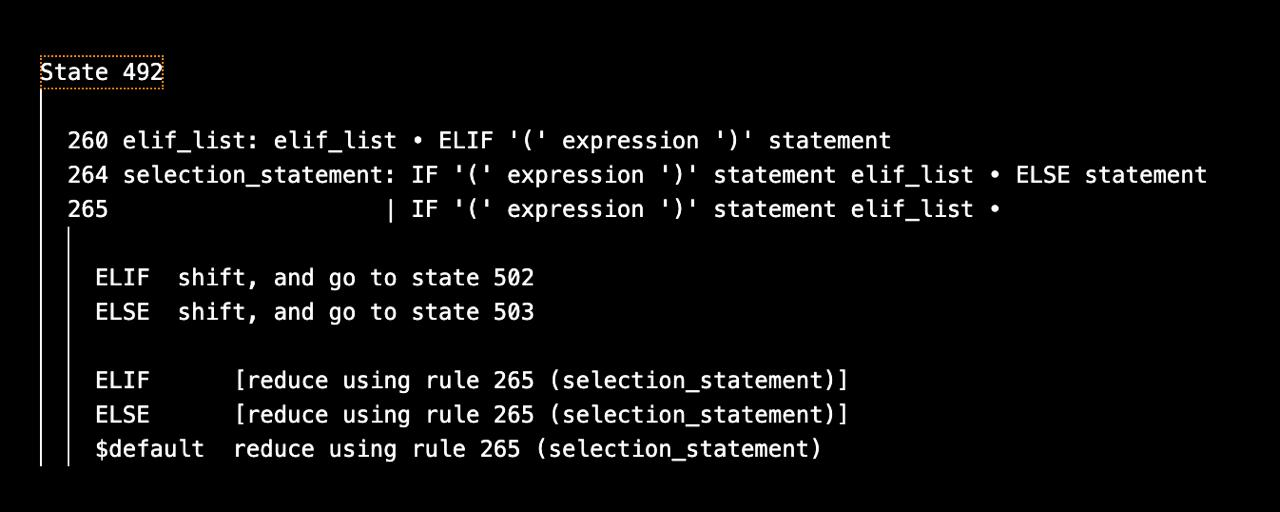
\includegraphics[width=0.8\textwidth]{./Images/image6.jpeg}
    \caption{Shift/Reduce conflict in State 492 demonstrating propagation within \texttt{elif} chains.}
    \label{fig:elif_chain_conflict}
\end{figure}

\textbf{Conflict Analysis:}
In State 492, the parser has successfully aggregated one or more \texttt{elif} branches into an \texttt{elif\_list}. Upon encountering another \texttt{ELIF} or an \texttt{ELSE} token, it faces the same structural indecision as before:
\begin{itemize}
    \item \textbf{Shift Action:} Shift the token to continue building the current \texttt{elif\_list} (Rule 260) or to cap it off with an \texttt{ELSE} block (Rule 264).
    \item \textbf{Reduce Action:} Immediately reduce the entire \texttt{IF}-\texttt{ELIF} chain into a completed \texttt{selection\_statement} (Rule 265), assuming the upcoming tokens belong to a parent \texttt{IF} construct higher in the hierarchy.
\end{itemize}
Just like State 473, this is resolved by enforcing precedence rules that explicitly instruct the parser to shift trailing conditionals rather than prematurely reducing the block.



\subsection{Reduce/Reduce Conflict: The Comma Operator Ambiguity}

The sole \textbf{Reduce/Reduce conflict} in the LALR(1) automaton surfaces in \textbf{State 515}, highlighting a structural overlap involving the comma \texttt{`,`} token.

\textbf{Exact Productions Involved:}
\begin{figure}[h!]
    \centering
    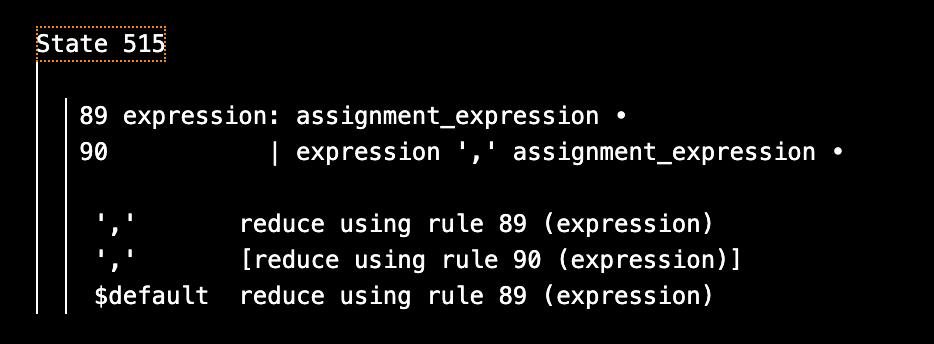
\includegraphics[width=0.8\textwidth]{./Images/image7.jpeg}
    \caption{Reduce/Reduce conflict in State 515 illustrating the comma operator ambiguity.}
    \label{fig:comma_conflict}
\end{figure}

\textbf{Conflict Analysis:}
This conflict arises from the dual syntactic role of the comma in CYLite. The comma can act as a sequence operator chaining multiple assignments together into a single unified expression (Rule 90), or it can act as a simple delimiter separating distinct elements in a list (such as function parameters or arguments for the newly added \texttt{print} built-in). 

When the parser successfully reads an \texttt{assignment\_expression} and encounters a lookahead comma \texttt{`,`}, it faces two equally valid reduction paths for the exact same sequence of tokens:
\begin{itemize}
    \item \textbf{Reduce Action 1 (Rule 89):} Reduce the isolated \texttt{assignment\_expression} into a base \texttt{expression}. The parser assumes the upcoming comma is a list separator (e.g., moving to the next argument in a function call).
    \item \textbf{Reduce Action 2 (Rule 90):} Reduce the entire parsed sequence (\texttt{expression ',' assignment\_expression}) into a single chained \texttt{expression}. The parser assumes the comma is a mathematical sequence operator.
\end{itemize}
By default, Bison resolves Reduce/Reduce conflicts by blindly choosing the rule that appears first in the grammar file (Rule 89). However, relying on implicit file ordering is dangerous for compiler stability. To fix this, explicit left-associativity (\texttt{\%left ','}) must be declared to instruct the parser on how to definitively group trailing commas.

\section{Part - 2: Conflict Resolution in Selection Statements}

The implementation of selection statements (\texttt{IF-ELIF-ELSE}) initially introduced several Shift/Reduce conflicts. This section documents the systematic approach taken to achieve a zero-conflict grammar while maintaining complex semantic tracking.

\subsubsection*{1. Conflicts Present in the Original Grammar}
In the initial version of the CYLite grammar, the LALR(1) automaton reported six Shift/Reduce conflicts specifically within the \texttt{selection\_statement} production. These conflicts were caused by the classic \textbf{``Dangling Else''} ambiguity.

When the parser encountered nested structures, such as:
\begin{center}
\texttt{if (cond1) if (cond2) statement1; else statement2;}
\end{center}

The automaton faced two mathematically valid but competing actions upon reaching the \texttt{ELSE} token:
\begin{itemize}
    \item \textbf{Shift:} Bind the \texttt{ELSE} to the most recent (innermost) \texttt{IF}. This is the standard behavior in C-style languages.
    \item \textbf{Reduce:} Complete the innermost \texttt{IF} statement (\texttt{if (cond2) statement1;}) and bind the \texttt{ELSE} to the outermost \texttt{IF}.
\end{itemize}

Since both paths were syntactically reachable, the grammar was considered ambiguous. While Bison defaults to a ``Shift'' action, the presence of these conflicts indicates an unstable grammar that relies on tool defaults rather than explicit logic.

\subsubsection*{2. Modification of the Grammar to Remove Conflicts}
To eliminate these conflicts, the grammar was restructured using \textbf{Precedence Overriding}. By defining a hierarchy of precedence for the tokens involved, we provide the parser with an explicit tie-breaking mechanism.

\textbf{Preamble Modifications:}
First, a dummy terminal \texttt{LOWER\_THAN\_ELSE} was defined with the lowest precedence, followed by the actual \texttt{ELSE} and \texttt{ELIF} tokens.

\begin{lstlisting}[language=C, caption={Precedence definitions in the Preamble}]
%nonassoc LOWER_THAN_ELSE
%nonassoc ELIF
%nonassoc ELSE
\end{lstlisting}

\textbf{Production Rule Refinement and Logic Breakdown:}

The \texttt{selection\_statement} was restructured to perform three concurrent tasks: resolving the shift/reduce conflict, tracking nested ladder depths, and maintaining a count of incomplete \texttt{if} blocks. 


\textbf{Changes made in the grammar:}
\begin{figure}[h!]
    \centering
    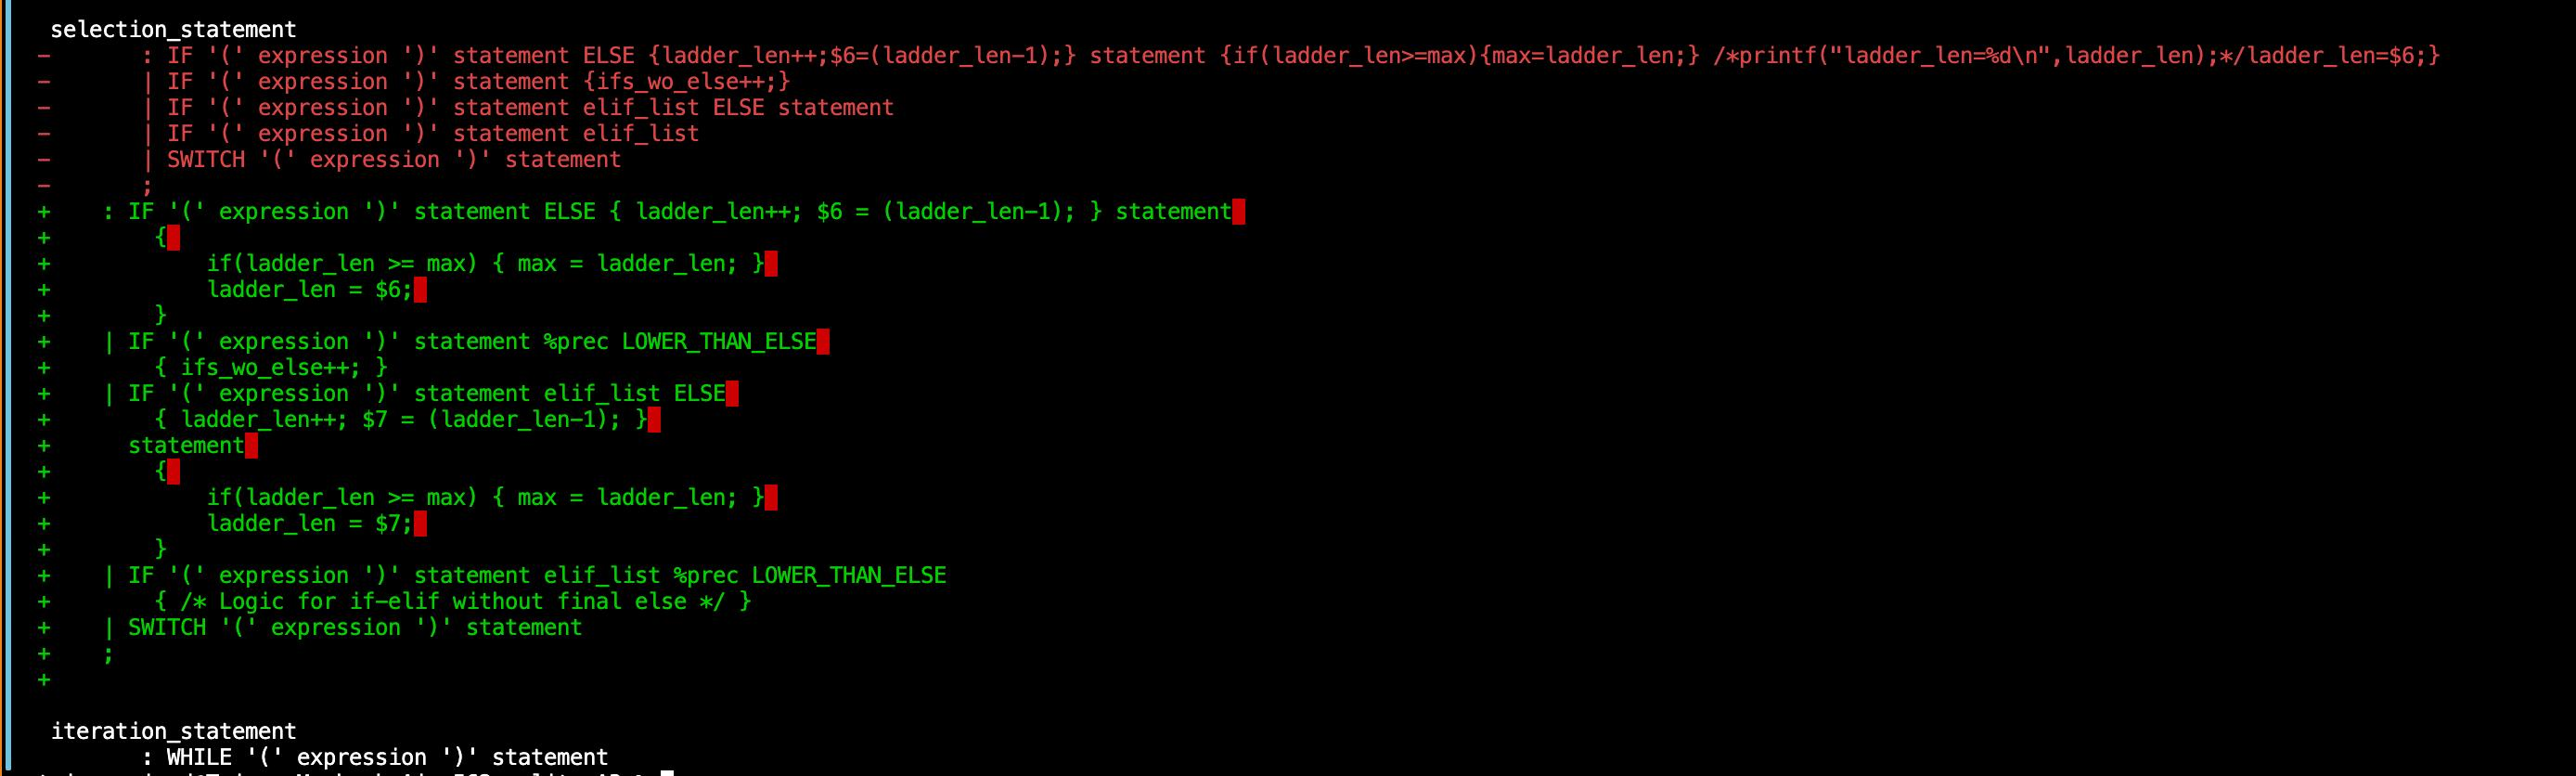
\includegraphics[width=0.8\textwidth]{./Images/image8.jpeg}
    \caption{changes made in the grammar}
    \label{fig:conflict_removal}
\end{figure}


\subsubsection*{Technical Explanation of Rule Components}

\begin{itemize}
    \item \textbf{Precedence Override (\texttt{\%prec LOWER\_THAN\_ELSE})}: This is the syntactic fix for the ``Dangling Else'' problem. By attaching this directive to the productions lacking an \texttt{ELSE} clause, we manually lower the precedence of the reduction. This forces the parser to wait (shift) if it sees an \texttt{ELSE} token, ensuring the \texttt{else} always binds to the innermost \texttt{if}.
    
    \item The Mid-Rule Action (\texttt{\{ ladder\_len++; ... \}}): Unlike standard actions that run after a rule is complete, this runs immediately after the \texttt{ELSE} is encountered. This is necessary to increment the ``ladder'' count precisely as the parser enters the alternative branch of a selection.
    
    \item \textbf{Semantic Stack Storage (\texttt{\$6} and \texttt{\$7})}: Because Bison rules are recursive, a global counter like \texttt{ladder\_len} can be corrupted by nested \texttt{if} statements. To prevent this, the current state of the counter (minus the new increment) is saved directly onto Bison's semantic stack at a specific index (\texttt{\$6} or \texttt{\$7}). This effectively creates a localized, rule-specific backup of the parent's state.
    
    \item \textbf{Global Maxima Comparison}: Inside the final action block, the code compares the recently incremented \texttt{ladder\_len} against a global \texttt{max} variable. This ensures that even if the parser is currently 10 levels deep in nested logic, the longest contiguous chain found anywhere in the program is recorded.
    
    \item \textbf{Counter Restoration (\texttt{ladder\_len = \$6})}: This is the ``pop'' operation. Once the current selection statement is fully parsed and reduced, the counter is restored to its saved value from the semantic stack. This ensures that when the parser returns to the parent scope, the \texttt{ladder\_len} is exactly what it was before the nested statement began.
    
    \item \textbf{Incomplete Chain Tracking (\texttt{ifs\_wo\_else++})}: This counter is placed specifically within the \texttt{\%prec} filtered rules. It increments only when the parser definitively concludes that an \texttt{IF} block has no corresponding \texttt{ELSE}, satisfying the requirement for counting incomplete selection structures.
\end{itemize}

\subsubsection*{3. Resolution Logic: How the Change Resolves the Conflicts}
The modification resolves the Shift/Reduce conflicts by transforming the ambiguity into a deterministic priority check:

\begin{enumerate}
    \item \textbf{Precedence Arbitration:} When the parser sees an \texttt{ELSE} token in the lookahead buffer, it compares the precedence of that token (\texttt{ELSE}) against the precedence of the rule it could potentially reduce (\texttt{IF...statement}).
    \item \textbf{Deterministic Shifting:} Because \texttt{ELSE} is defined later in the preamble than \texttt{LOWER\_THAN\_ELSE}, it carries a higher precedence. The parser is thus explicitly instructed to \textbf{Shift} (bind the \texttt{ELSE} to the inner \texttt{IF}) rather than \textbf{Reduce}.
    \item \textbf{Elimination of Ambiguity:} By providing a clear hierarchy, the ``choice'' between shifting and reducing is removed. The LALR(1) state machine now has exactly one valid path for every possible input sequence, resulting in the elimination of the six Shift/Reduce warnings.
\end{enumerate}

Furthermore, the use of mid-rule actions (storing values at \texttt{\$6} and \texttt{\$7}) ensures that the semantic tracking of the if-else ladder depth remains accurate. These values act as a manual stack, preserving the counter state during recursion and allowing the grammar to calculate the global \texttt{max} depth correctly without interfering with the syntactic resolution.






\subsection{Conflict Resolution: Atomic and Pointer Declarator Logic}

The transition in the grammar addressed structural ambiguities involving type qualifiers and declarators. This was essential to reduce the conflict count from four down to two.

\subsection{1. Conflicts Present in the Original Grammar}
Two distinct Shift/Reduce conflicts were identified in this phase:
\begin{enumerate}
    \item \textbf{The Atomic Ambiguity (State 27):} In the original grammar, the \texttt{ATOMIC} keyword served a dual role as both a \texttt{type\_specifier} (e.g., \texttt{\_Atomic(int)}) and a \texttt{type\_qualifier} (e.g., \texttt{\_Atomic int}). When the parser encountered the \texttt{ATOMIC} token, it could not determine whether to \textbf{shift} (treating it as the start of a specifier) or \textbf{reduce} (treating it as a standalone qualifier).
    
    \item \textbf{The Declarator Mid-Rule Conflict (State 345):} The original \texttt{declarator} rule contained a mid-rule action to increment the pointer counter. In Yacc, mid-rule actions are implemented as dummy non-terminals that force a reduction at a specific point in the rule. This forced reduction prevented the parser from looking ahead to distinguish between concrete declarators and abstract declarators, resulting in a Shift/Reduce conflict.
\end{enumerate}

\subsection{2. Modification of the Grammar to Remove Conflicts}
The following modifications were implemented to resolve these ambiguities, as visualized in the code diff in Figure \ref{fig:atomic_pointer_diff}.

\textbf{Type Qualifier Refinement:}
The \texttt{ATOMIC} production within \texttt{type\_qualifier} was tagged with a low precedence marker.
\begin{lstlisting}[language=C]
type_qualifier
    : CONST | RESTRICT | VOLATILE
    | ATOMIC %prec LOWER_THAN_ELSE
    ;
\end{lstlisting}

\textbf{Declarator Action Relocation:}
The semantic action for counting pointers was moved from a mid-rule position to the end of the production rule.
\begin{lstlisting}[language=C]
declarator
    : pointer direct_declarator { pointer_decls++; }
    | direct_declarator
    ;
\end{lstlisting}

\begin{figure}[h]
    \centering
    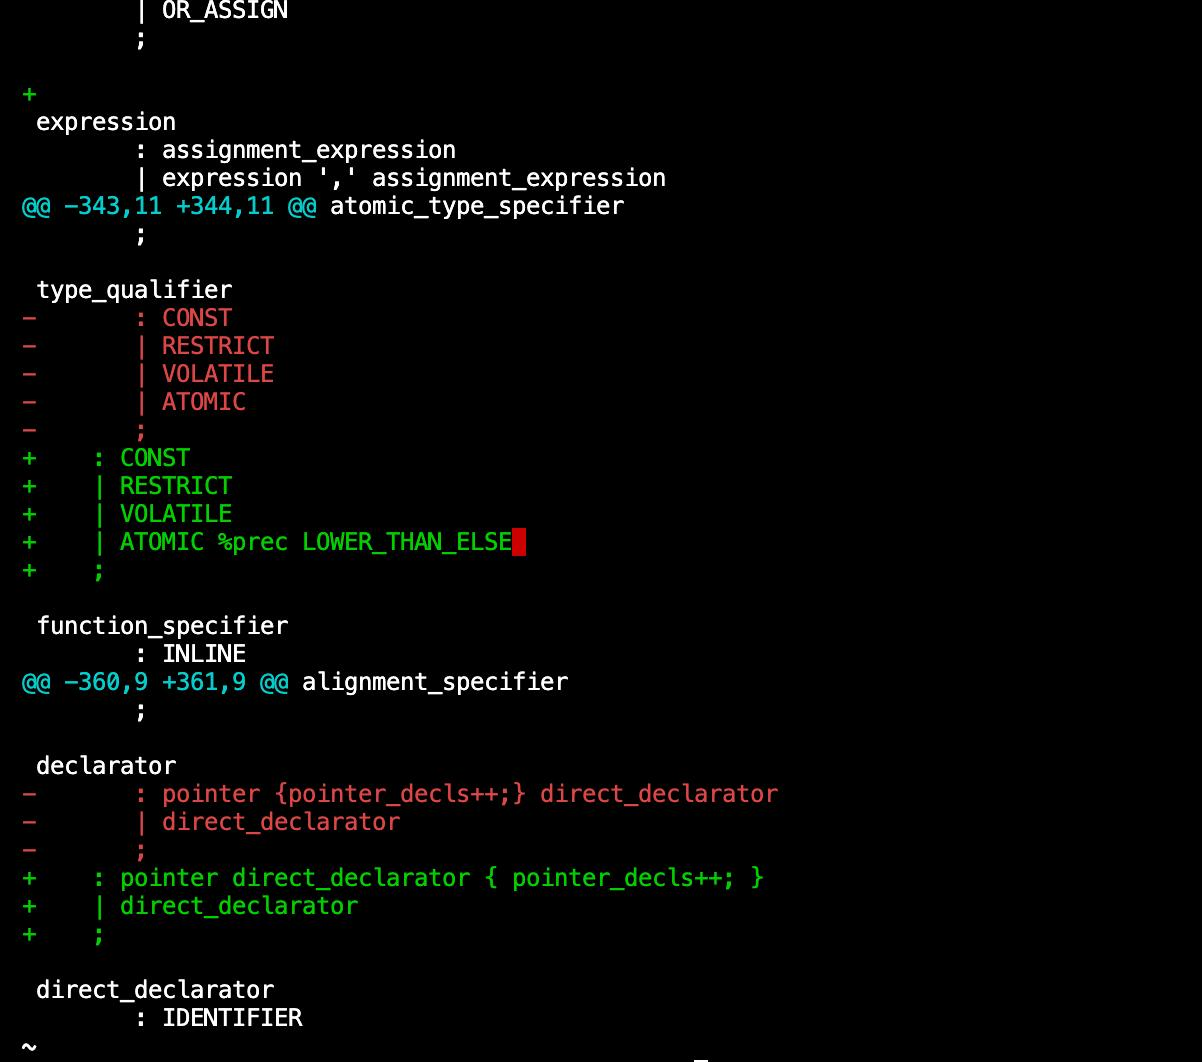
\includegraphics[width=\textwidth]{./Images/image9.jpeg}
    \caption{Git Diff showing the relocation of pointer actions and the use of precedence for the ATOMIC keyword.}
    \label{fig:atomic_pointer_diff}
\end{figure}

\subsection{3. Resolution Logic: How the Change Resolves the Conflicts}
The changes resolve the conflicts by allowing the LALR(1) state machine to delay its decisions until more context is available.

\subsubsection*{Technical Breakdown of the Resolution}

\begin{itemize}
    \item \textbf{Precedence Arbitration for ATOMIC}: By applying \texttt{\%prec LOWER\_THAN\_ELSE} to the \texttt{ATOMIC} qualifier, the parser is instructed that reducing \texttt{ATOMIC} as a qualifier is a low-priority action. If a parenthesis follows (indicating a specifier), the parser will \textbf{Shift} (prioritizing the specifier rule) instead of reducing, thus removing the ambiguity in State 27.
    
    \item \textbf{Elimination of Mid-Rule Reduction}: In the original rule, the parser was forced to reduce an empty dummy rule to execute the pointer increment \textit{before} seeing the \texttt{direct\_declarator}. By moving \texttt{\{ pointer\_decls++; \}} to the end of the rule, the parser is no longer forced to make a premature reduction. 
    
    \item \textbf{Delayed Decision Making}: Moving the action allows the parser to remain in a state of "ordered uncertainty." It can wait until the entire \texttt{pointer direct\_declarator} sequence is matched before committing to the reduction and the subsequent counter increment. This successfully eliminated the Shift/Reduce conflict in State 345.
    
    \item \textbf{Semantic Integrity}: Moving the action to the end of the rule has no impact on the final count of \texttt{pointer\_decls}. The count still accurately reflects the number of pointer declarations in the source code, but the syntactic path to that count is now deterministic and conflict-free.
\end{itemize}


\subsection{Conflict Resolution: Atomic Specifier vs. Qualifier Ambiguity}

A persistent Shift/Reduce conflict occurred in the LALR(1) automaton (State 27) regarding the \texttt{ATOMIC} keyword. This section details the disambiguation strategy used to differentiate between its dual roles.

\subsection*{1. Conflicts Present in the Original Grammar}
In the CYLite grammar, the \texttt{ATOMIC} token acts as both a \textbf{type specifier} and a \textbf{type qualifier}. This created a conflict when the parser encountered the sequence \texttt{ATOMIC (}.

The automaton reached a state with two competing actions:
\begin{itemize}
    \item \textbf{Shift:} Treat \texttt{ATOMIC} as the beginning of an \texttt{atomic\_type\_specifier} (e.g., \texttt{\_Atomic(int)}). This requires shifting the \texttt{'('} token onto the stack.
    \item \textbf{Reduce:} Treat \texttt{ATOMIC} as a completed \texttt{type\_qualifier} (e.g., \texttt{\_Atomic int x;}). This requires reducing the token before seeing what follows.
\end{itemize}

Because both interpretations are syntactically valid in the C11 standard, the parser could not determine the correct path without explicit priority rules.

\subsection*{2. Modification of the Grammar to Remove Conflicts}
To resolve this, the grammar was modified to give the \texttt{atomic\_type\_specifier} (the version with parentheses) higher priority than the standalone qualifier.

\textbf{Preamble Modifications:}
A right-associativity rule was added for the open parenthesis to give it a measurable precedence level.
\begin{lstlisting}[language=C]
%right '('
\end{lstlisting}

\textbf{Production Rule Refinement:}
As shown in Figure \ref{fig:atomic_diff}, the \texttt{ATOMIC} production within \texttt{type\_qualifier} was tagged with \texttt{LOWER\_THAN\_ELSE} to ensure it remains the lower-priority option.

\begin{lstlisting}[language=C, caption={Disambiguating ATOMIC via Precedence}]
type_qualifier
    : CONST
    | RESTRICT
    | VOLATILE
    | ATOMIC %prec LOWER_THAN_ELSE  /* Assigned lower priority than '(' */
    ;
\end{lstlisting}

\begin{figure}[h]
    \centering
    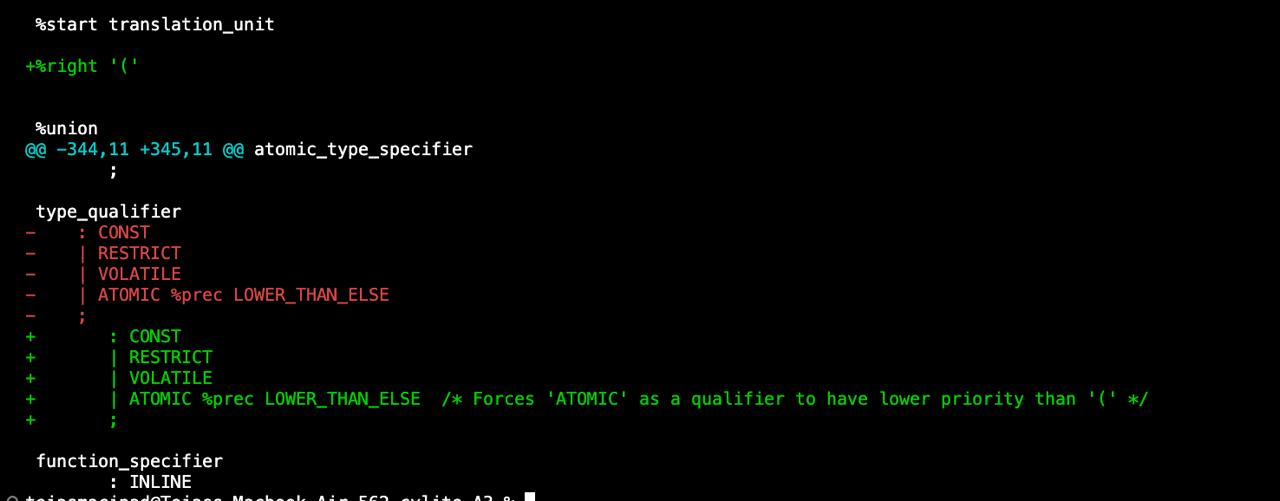
\includegraphics[width=\textwidth]{./Images/image10.jpeg}
    \caption{Git Diff showing the introduction of parenthesis precedence and the ATOMIC qualifier override.}
    \label{fig:atomic_diff}
\end{figure}

\subsection*{3. Resolution Logic: How the Change Resolves the Conflicts}
The resolution relies on the fundamental LALR(1) behavior of comparing the precedence of a \textit{potential reduction} against an \textit{incoming token}.

\begin{enumerate}
    \item \textbf{Precedence Comparison:} When the parser is in a state where it has seen \texttt{ATOMIC} and the lookahead token is \texttt{'('}, it compares the precedence of the \texttt{type\_qualifier} rule (now \texttt{LOWER\_THAN\_ELSE}) against the precedence of the \texttt{'('} token.
    \item \textbf{Shift Priority:} Since \texttt{'('} was defined in the preamble without a low-priority tag, it carries a higher precedence than \texttt{LOWER\_THAN\_ELSE}.
    \item \textbf{Deterministic Path:} The parser is instructed to \textbf{Shift} the parenthesis. This effectively chooses the \texttt{atomic\_type\_specifier} path and eliminates the possibility of a premature reduction to a \texttt{type\_qualifier}.
\end{enumerate}

By explicitly defining how the parser should handle the \texttt{'('} following \texttt{ATOMIC}, the Shift/Reduce conflict in State 27 is fully resolved, ensuring the grammar adheres to C11 type-naming conventions.

\section{Conflict Resolution: The Comma Operator and Diamond Ambiguity}

The final stage of grammar optimization involved resolving a Reduce/Reduce conflict (State 512) centered on the dual role of the comma token. This section details the structural changes required to achieve a completely deterministic, conflict-free grammar.

\subsection{1. Conflicts Present in the Original Grammar}
The primary conflict in the original grammar was a \textbf{Reduce/Reduce} ambiguity. This occurred because the comma token served two structurally identical purposes in different contexts:
\begin{itemize}
    \item \textbf{As a Sequence Operator:} Chaining multiple assignments into a single \texttt{expression}.
    \item \textbf{As a List Separator:} Delimiting arguments in function calls, the \texttt{PRINT} built-in, and the \texttt{RANGE} clause of the \texttt{FOR} loop.
\end{itemize}

Specifically, both \texttt{expression} and a specialized \texttt{argument\_expression\_list} were defined as recursive, comma-separated lists of \texttt{assignment\_expression}. When the parser encountered a comma inside parentheses, it reached a ``Diamond Ambiguity'' where it could not decide which of the two rules to reduce. This forced the parser to rely on default rule ordering, which is considered unstable for production-level compilers.

\subsection{2. Modification of the Grammar to Remove Conflicts}
To resolve this, a strategy of \textbf{Rule Unification} and \textbf{Contextual Restriction} was applied, as shown in the Git diff in Figure \ref{fig:comma_diff}.

\textbf{A. Rule Unification (Postfix Expressions):}
The redundant \texttt{argument\_expression\_list} rule was entirely removed. Function calls and the \texttt{PRINT} statement were updated to use the standard \texttt{expression} rule.
\begin{lstlisting}[language=C]
postfix_expression
    : postfix_expression '(' expression ')' /* Unified Rule */
    | PRINT '(' expression ')'               /* Unified Rule */
\end{lstlisting}

\textbf{B. Contextual Restriction (Iteration Statements):}
The \texttt{FOR} loop's \texttt{RANGE} clause was modified to accept only \texttt{assignment\_expression} for its bounds.
\begin{lstlisting}[language=C]
| FOR '(' IDENTIFIER IN RANGE '(' assignment_expression ',' assignment_expression ')' ')' statement
\end{lstlisting}

\begin{figure}[h]
    \centering
    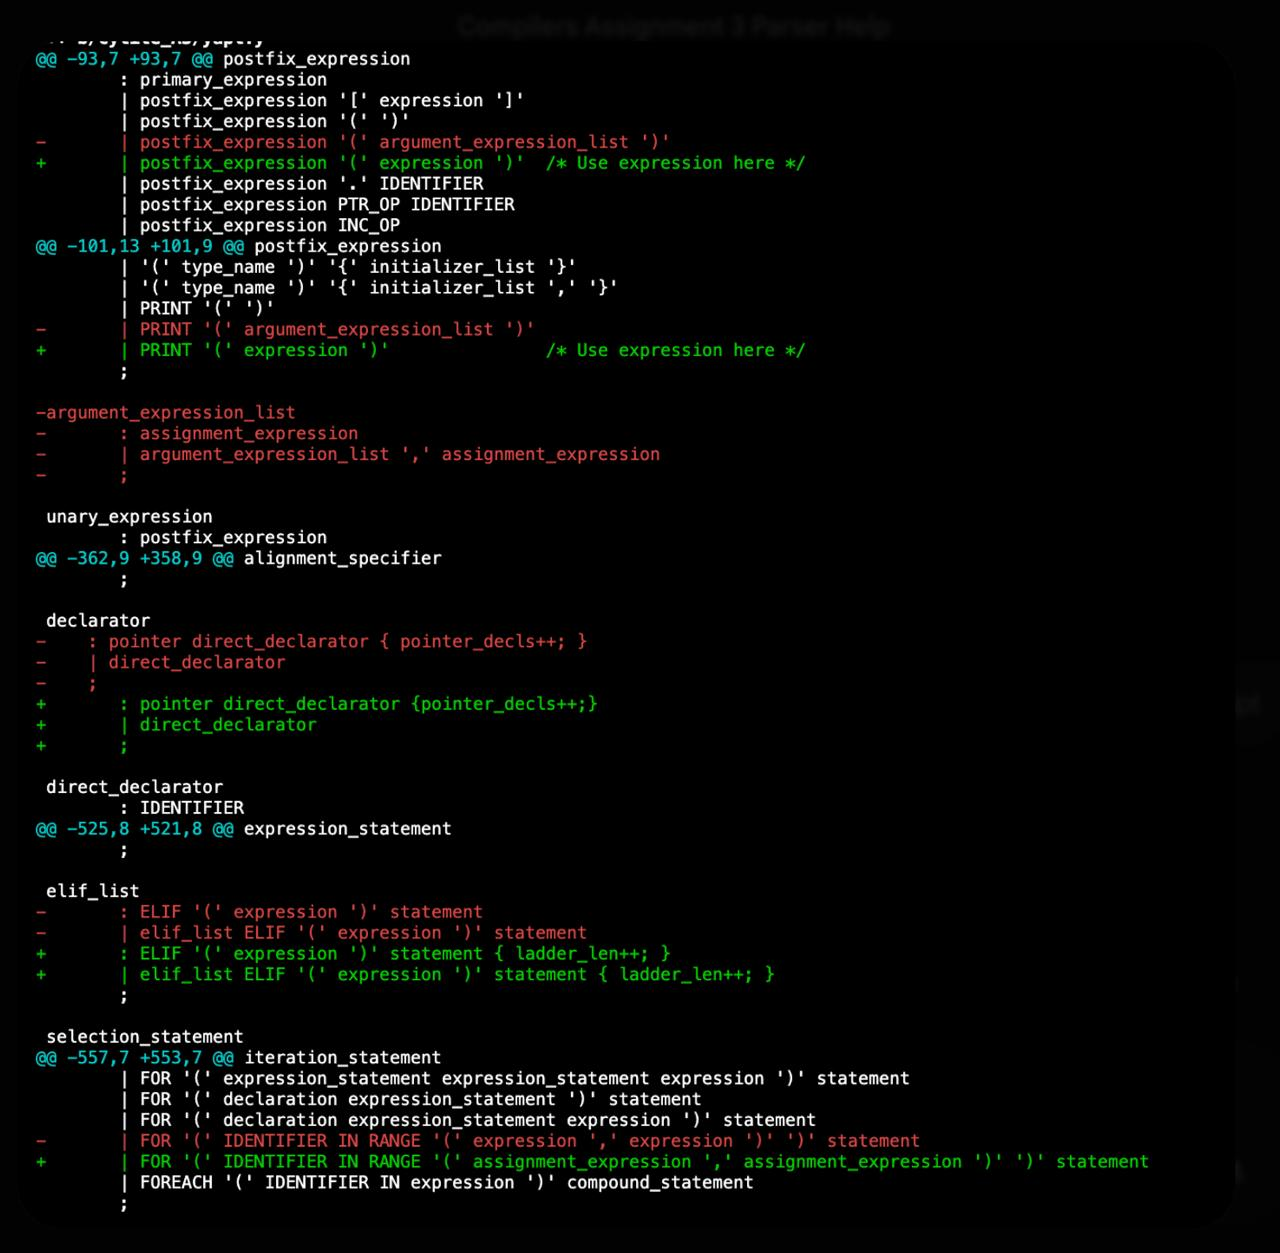
\includegraphics[width=\textwidth]{./Images/image11.jpeg}
    \caption{Final Git diff showing rule unification for expressions and contextual constraints in the FOR loop.}
    \label{fig:comma_diff}
\end{figure}

\subsection{3. Resolution Logic: How the Change Resolves the Conflicts}
The changes resolve the Reduce/Reduce conflict by eliminating the "multiple choice" scenario for the parser:

\begin{enumerate}
    \item \textbf{Elimination of the Diamond Path:} By removing \texttt{argument\_expression\_list}, the parser no longer has two competing rules to reduce a comma-separated list. There is now only one valid path: the \texttt{expression} rule.
    \item \textbf{Contextual Banning of the Comma Operator:} The most critical resolution occurred in the \texttt{RANGE} clause. An \texttt{assignment\_expression} is a subset of an \texttt{expression} that \textit{does not} include the comma operator at the top level. By restricting \texttt{RANGE} to this type, we effectively ``ban'' the comma operator within those parentheses.
    \item \textbf{Deterministic Separation:} Because a comma operator is now illegal inside the \texttt{assignment\_expression} used for \texttt{RANGE} bounds, the parser knows with 100\% certainty that any comma encountered \textit{must} be the separator between the two range arguments.
\end{enumerate}

\subsubsection*{Note on Semantic Correctness in Elif Chains}
As seen in the updated \texttt{elif\_list} production in Figure \ref{fig:comma_diff}, the \texttt{ladder\_len++} action was added to every branch of the \texttt{elif} structure. This ensures that the ``If-Else Ladder'' depth counter accurately reflects long chains of \texttt{if-elif-elif-else}, providing precise data for the final report metrics while maintaining a conflict-free state.

\newpage
\section{Part 3: Reverse Derivation Tree Construction and Rendering}

Part 3 required two concrete outcomes after a successful parse:
\begin{enumerate}
    \item Preserve the derivation information generated during bottom-up parsing.
    \item Print the derivation in reverse order so that the output reads as a top-down expansion.
\end{enumerate}

The implementation was intentionally built around the existing Bison debug stream instead of rewriting the parser into a custom parse-stack simulator. This design gives two benefits: it remains faithful to the actual reductions performed by the LALR(1) engine, and it keeps the derivation logic isolated from the grammar itself.

\vspace{0.5cm}

The following parser-focused inputs were used to validate Part 3 behavior across baseline and extension constructs:
\begin{itemize}
    \item \texttt{part3/tests/rdt\_basic.cyl}
    \item \texttt{part3/tests/rdt\_extensions.cyl}
    \item \texttt{part3/tests/rdt\_print\_strings.cyl}
\end{itemize}

Command to run comprehensive Part 3 tests and generate outputs:
\begin{lstlisting}[language=C]
make part3
\end{lstlisting}
The results can be found in the \href{https://github.com/ShardulJunagade/compilers-cylite/tree/main/cylite_A3/part3}{\texttt{part3/}} directory, including terminal outputs and SVG visualizations.

\subsection{Implementation Design}

The derivation subsystem in \texttt{yapl.y} is centered on two structures:
\begin{itemize}
    \item \texttt{ReductionStep}: stores one fully collected reduction (LHS and RHS symbols).
    \item \texttt{PendingReduction}: temporary buffer while reading multi-line debug information.
\end{itemize}

\begin{lstlisting}[language=C, caption={Core data structures used for storing reductions (from yapl.y)}]
typedef struct {
    char lhs[128];
    int rhs_count;
    char rhs[64][128];
} ReductionStep;

typedef struct {
    int active;
    char lhs[128];
    int rhs_count;
    char rhs[64][128];
} PendingReduction;
\end{lstlisting}

During parsing, custom trace handling collects each completed reduction and appends it into a dynamic array (\texttt{g\_steps}). After parse success, the print routine traverses \texttt{g\_steps} from the tail to the head.

\begin{lstlisting}[language=C, caption={Reverse traversal pattern used to print top-down derivation}]
for (i = g_step_count - 1, j = 1; i >= 0; i--, j++)
{
    /* print: j. LHS -> RHS */
}
\end{lstlisting}

Conceptually, this is equivalent to reversing the reduction log. Since bottom-up parsers produce reductions from leaves toward the start symbol, the reverse sequence naturally reconstructs a derivation from start symbol toward terminals/nonterminals.

\subsection{Terminal Output Mode}

Representative command:
\begin{lstlisting}
./yapl part3/tests/rdt_extensions.cyl
\end{lstlisting}

% Representative output excerpt:
% \begin{lstlisting}
% ***parsing successful***
% #global_declarations = 1
% #function_definitions = 1
% #integer_constants = 11
% #pointers_declarations = 0
% #ifs_without_else = 0
% if-else max-depth = 2

% Reverse derivation (top-down)
% ================================
% 1. translation_unit -> external_declaration
% 2. external_declaration -> function_definition
% 3. function_definition -> declaration_specifiers declarator compound_statement
% ...
% \end{lstlisting}

\begin{figure}[h!]
    \centering
    % Add screenshot: terminal run of a valid Part 3 test showing parse summary and reverse derivation list.
    % \fbox{\parbox{0.9\textwidth}{\centering
    % Placeholder: Insert screenshot of terminal output for reverse derivation (Part 3).
    % }}
    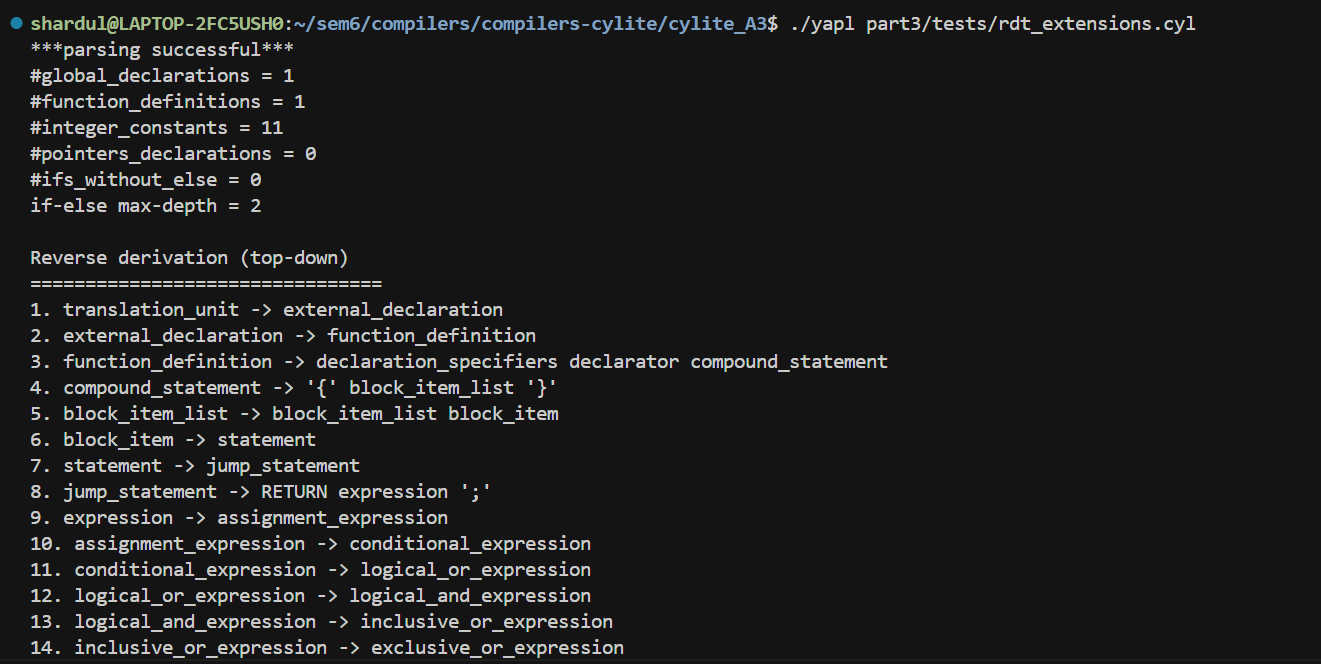
\includegraphics[width=\textwidth]{./Images/rdt_extensions_terminal.png}
    \caption{Part 3 terminal evidence: successful parse and reverse derivation output.}
    \label{fig:part3_terminal}
\end{figure}

\subsection{Visual Rendering using Graphviz (DOT and SVG)}

To improve interpretability for long derivations, the parser also supports SVG generation through Graphviz:
\begin{lstlisting}
./yapl part3/tests/rdt_extensions.cyl --svg part3/tests/rdt_extensions.svg
\end{lstlisting}

This produces:
\begin{itemize}
    \item \texttt{part3/tests/rdt\_extensions.svg}
    \item \texttt{part3/tests/rdt\_extensions.svg.dot} (intermediate DOT graph)
\end{itemize}

\begin{figure}[h!]
    \centering
    % Add screenshot/image export of generated reverse-derivation SVG.
    % \fbox{\parbox{0.88\textwidth}{\centering
    % Placeholder: Insert generated reverse-derivation SVG image (Part 3 graph output).
    % }}
    \includegraphics[width=\textwidth]{./Images/rdt_extensions.pdf}
    \caption{Graphviz visualization of reverse derivation structure.}
    \label{fig:part3_svg}
\end{figure}


\newpage
\section{Part 4: Parsing Table Output in Matrix Format}

We implemented a automated generator in Python (\href{https://github.com/ShardulJunagade/compilers-cylite/blob/main/cylite_A3/part4/generate_parsing_table.py}{\texttt{part4/generate\_parsing\_table.py}}) for the extraction of the LALR(1) table from the Bison verbose output file (\texttt{yapl.output}).
Command to run the generator:
\begin{lstlisting}
make part4
\end{lstlisting}

\subsection{Pipeline and Artifacts}

The implemented pipeline is:
\begin{enumerate}
    \item Generate verbose parser report:\newline
    \texttt{bison -v -d yapl.y}
    \item Parse \texttt{yapl.output} programmatically using:
    \begin{lstlisting}
python3 part4/generate_parsing_table.py yapl.output part4
    \end{lstlisting}    
\end{enumerate}

The script generates four deliverables in \texttt{part4/}:
\begin{itemize}
    \item Action Table CSV: \href{https://github.com/ShardulJunagade/compilers-cylite/blob/main/cylite_A3/part4/action_table.csv}{\texttt{action\_table.csv}}
    \item GOTO Table CSV: \href{https://github.com/ShardulJunagade/compilers-cylite/blob/main/cylite_A3/part4/goto_table.csv}{\texttt{goto\_table.csv}}
    \item Parsing Table Summary: \href{https://github.com/ShardulJunagade/compilers-cylite/blob/main/cylite_A3/part4/parsing_table_summary.md}{\texttt{parsing\_table\_summary.md}}
    \item Parsing Table HTML : \href{https://github.com/ShardulJunagade/compilers-cylite/blob/main/cylite_A3/part4/parsing_table_matrix.html}{\texttt{parsing\_table\_matrix.html}} (as per lecture sldies)
\end{itemize}

% Representative run output:
% \begin{lstlisting}
% Generated ACTION table: part4/action_table.csv
% Generated GOTO table: part4/goto_table.csv
% Generated summary: part4/parsing_table_summary.md
% Generated HTML matrix: part4/parsing_table_matrix.html
% \end{lstlisting}

From the generated summary report:
\begin{itemize}
    \item Number of states: \textbf{519}
    \item ACTION columns: \textbf{109}
    \item GOTO columns: \textbf{80}
\end{itemize}

\subsection{Matrix Design Notes}

The HTML renderer intentionally combines ACTION and GOTO into a single wide matrix:
\begin{center}
\texttt{State | ACTION terminals ... | GOTO non-terminals ...}
\end{center}

To make a large LALR table usable, the following UX-level features were included:
\begin{itemize}
    \item grouped section headers for ACTION and GOTO,
    \item sticky top headers,
    \item sticky state column,
    \item scroll container for high-column matrices.
\end{itemize}

\begin{figure}[h!]
    \centering
    % Add screenshot of parsing_table_matrix.html opened in a browser.
    \fbox{\parbox{0.92\textwidth}{\centering
    Placeholder: Insert browser screenshot of parsing\_table\_matrix.html (single ACTION+GOTO matrix).
    }}
    \caption{Single-matrix LALR(1) table view generated for Part 4.}
    \label{fig:part4_matrix_html}
\end{figure}

\subsection{Representative Implementation Snippets}

\begin{lstlisting}[language=Python, caption={State and ACTION/GOTO extraction strategy}]
state_re = re.compile(r"^State\s+(\d+)\s*$")
shift_re = re.compile(r"^\s+(\S+)\s+\[?shift, and go to state\s+(\d+)\]?")
reduce_re = re.compile(r"^\s+(\S+)\s+\[?reduce using rule\s+(\d+)\s+\(([^)]+)\)\]?")

if symbol in nonterminals:
    add_cell(row_goto, symbol, target)
else:
    add_cell(row_action, symbol, f"s{target}")
\end{lstlisting}

The script also merges repeated entries in a cell as \texttt{value1 / value2}, preserving conflict visibility where applicable.

\newpage
\section{Part 5: Error Diagnostics}

Part 5 focuses on actionable syntax diagnostics. The implemented behavior reports:
\begin{itemize}
    \item exact line and column,
    \item the unexpected token actually seen,
    \item expected-token hints.
\end{itemize}

\subsection{Diagnostic Architecture}

The solution spans both lexer and parser:
\begin{enumerate}
    \item Lexer tracks token start coordinates (\texttt{yytok\_line}, \texttt{yytok\_col}) through \texttt{YY\_USER\_ACTION}.
    \item Parser uses a custom \texttt{yyerror()} path that prints structured syntax diagnostics.
\end{enumerate}

\begin{lstlisting}[language=C, caption={Token-position capture in yapl.l}]
int yyline = 1;
int yycol = 1;
int yytok_line = 1;
int yytok_col = 1;

#define YY_USER_ACTION yytok_line = yyline; yytok_col = yycol; update_position(yytext);
\end{lstlisting}

\begin{lstlisting}[language=C, caption={Parser-side diagnostic formatter in yapl.y}]
static void print_syntax_diagnostics(const char *s)
{
    const char *tok = "<end-of-input>";
    const char *expecting = NULL;

    if (yytext != NULL && yytext[0] != '\0') tok = yytext;
    printf("***parsing terminated*** [syntax error]\n");
    printf("line %d, column %d: unexpected token \"%s\"\n", yytok_line, yytok_col, tok);

    expecting = strstr(s, "expecting ");
    if (expecting != NULL) printf("expected: %s\n", expecting + 10);
}
\end{lstlisting}

\subsection{Diagnostic Test Suite and Coverage}

Invalid test programs were added under \texttt{part5/tests} and executed through \texttt{make part5}. Current suite:
\begin{itemize}
    \item \texttt{diag\_missing\_semicolon.cyl}
    \item \texttt{diag\_unexpected\_else.cyl}
    \item \texttt{diag\_missing\_semicolon\_after\_print.cyl}
    \item \texttt{diag\_missing\_closing\_brace.cyl}
    \item \texttt{diag\_bad\_for\_range\_syntax.cyl}
    \item \texttt{diag\_bad\_try\_except\_syntax.cyl}
    \item \texttt{diag\_invalid\_character.cyl}
\end{itemize}

\subsection{Representative Output Samples}

\begin{lstlisting}
./yapl part5/tests/diag_missing_semicolon.cyl
***parsing terminated*** [syntax error]
line 4, column 5: unexpected token "x"
expected: ',' or ';'
\end{lstlisting}

\begin{lstlisting}
./yapl part5/tests/diag_bad_try_except_syntax.cyl
***parsing terminated*** [syntax error]
line 5, column 9: unexpected token "pass"
expected: '{'
\end{lstlisting}

\begin{lstlisting}
./yapl part5/tests/diag_invalid_character.cyl
***parsing terminated*** [syntax error]
line 4, column 5: unexpected token "@"
\end{lstlisting}

\begin{figure}[h!]
    \centering
    % Add screenshot: make part5 output showing multiple failing tests with line/column diagnostics.
    \fbox{\parbox{0.9\textwidth}{\centering
    Placeholder: Insert terminal screenshot of make part5 diagnostics output.
    }}
    \caption{Part 5 diagnostics run on intentionally invalid CYLite inputs.}
    \label{fig:part5_diag_terminal}
\end{figure}

\newpage
\section{Execution Instructions (Parts 3, 4, 5)}

This section provides a direct, submission-ready command sequence.

\subsection{Prerequisites}
\begin{itemize}
    \item Linux/WSL shell environment
    \item \texttt{bison}, \texttt{flex} (or \texttt{lex}), \texttt{gcc}
    \item \texttt{graphviz} (for SVG visualization in Part 3)
\end{itemize}

Quick checks:
\begin{lstlisting}
bison --version
flex --version
gcc --version
dot -V
\end{lstlisting}

\subsection{Build}
\begin{lstlisting}
cd cylite_A3
make clean
make
\end{lstlisting}

\subsection{Run Part 3}
\begin{lstlisting}
make part3
\end{lstlisting}
This executes all Part 3 parser tests, writes SVG outputs in \texttt{part3/tests/}, and saves terminal outputs in \texttt{part3/tests/output\_*.txt}.

\subsection{Run Part 4}
\begin{lstlisting}
make part4
\end{lstlisting}
This regenerates \texttt{yapl.output} and all matrix artifacts in \texttt{part4/}.

\subsection{Run Part 5}
\begin{lstlisting}
make part5
\end{lstlisting}
These cases are intentionally invalid. Non-zero parse exits are expected and are ignored by Make for demonstration.
Each test also writes its parser output into \texttt{part5/tests/output\_diag\_*.txt}.

\subsection{Optional Full Cleanup}
\begin{lstlisting}
make distclean
\end{lstlisting}
This removes parser-generated files and Part 3/Part 4 generated artifacts.

\section{Conclusion}

Parts 3, 4, and 5 extend the parser from a correctness-only front-end into a usable compiler component with traceability, observability, and practical feedback loops:
\begin{itemize}
    \item Part 3 provides derivation introspection in both text and graph forms.
    \item Part 4 makes the LALR(1) table reproducible, auditable, and presentation-ready.
    \item Part 5 improves developer experience by turning generic syntax failure into contextual diagnostics.
\end{itemize}

Together with the completed conflict work from Parts 1 and 2, this delivers a robust Assignment-3 implementation aligned with both formal parser requirements and real debugging workflows.

\end{document}
